\subsection{Applications of Derivatives}

\subsubsection{Optimization}
Optimization uses maxima and minima to identify optimal solutions to problems given a restraint and equation.\\
Steps to solve:
\begin{enumerate}
    \item Define the relevant quantities
    \item Determine a formula in the form $f(x)$
    \item Find an interval of possible values from physical restrictions
    \item Take the derivative and find critical points
    \item Find the maximum/minimum values
\end{enumerate}
Ex: A rectangular enclosure is to be built with one side against a wall and 3 sides fenced. 100m of fence is available. What is the maximum possible area?
\begin{align*}
    &A=lw\\
    &P=100=2w+l\\
    &\Ra l=100-2w\\
    &A(w)=x(100-2x)=100-2x^2\\
    &\text{Restrictions: }w\geq 0,\, l\geq 0\Ra 100-2w\geq 0\Ra 0\leq w\leq 50\\
    &\frac{dA}{dw}=100-4w=0\Ra w=25\\
    &\text{Test critical points: }\\
    &A(0)=0\\
    &A(25)=1250\\
    &A(50)=0\\
    &\therefore \text{max area is }1250m^2
\end{align*}
Ex2: An IMAX movie screen is 16m tall, base 9m above eye level. How far from the screen is the "best" view? (goal: maximize $\theta$)\\
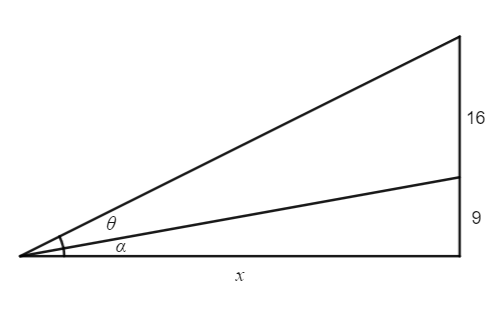
\includegraphics[scale=0.8]{DifferentialCalculusPictures/OptimizationEx.png}
\begin{align*}
    &\tan\alpha=\frac{9}{x}
    &\tan(\alpha+\theta)=\frac{25}{x}\\
    &\alpha=\arctan\brround{\frac{9}{x}}
    &\alpha+\theta=\arctan\brround{\frac{25}{x}}\\
    &\theta=\arctan\brround{\frac{25}{x}}-\arctan\brround{\frac{9}{x}}\\
    &\text{endpoints:}\\
    &\lim_{x\to0^+}\theta=\frac{\pi}{2}-\frac{\pi}{2}=0\\
    &\lim_{x\to\infty}\theta=0\\
    &\text{critical points:}\\
    &\theta'(x)=\frac{16(15^2-x^2)}{(x^2+9^2)(x^2+25^2)}\\
    &\Ra x=15
\end{align*}
Ex3: Find the volume of the largest cylinder that can be inscribed in a cone.\\
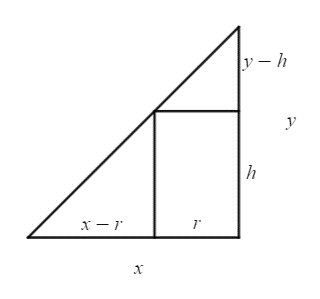
\includegraphics[scale=0.65]{DifferentialCalculusPictures/InscribedCylinder.png}
\begin{align*}
    &V=\pi r^2 h\\
    &\text{Using like triangles: }\frac{h}{x-r}=\frac{y}{x}\\
    &h=\frac{y(x-r)}{x}\\
    &V=\pi r^2\frac{y}{x}(x-r)=\pi r^2y-\pi r^3\frac{y}{x}\\
    &\text{*treat $x$ and $y$ as constants*}\\
    &2\pi ry-3\pi r^2\frac{y}{x}\\
    &\frac{dV}{dr}=2\pi ry\brround{2-\frac{3r}{x}}=0\Ra r=0,\,r=\frac{2x}{3}\\
    &h=\frac{y\brround{x-\frac{2x}{3}}}{x}=\frac{y}{3}\\
    &V=\pi\brround{\frac{2x}{3}}^2\brround{\frac{y}{3}}=\frac{4\pi}{27}x^2y
\end{align*}
We can also calculate the ratio of the two volumes to find that the volume of the cylinder is $\frac{4}{9}$ the volume of the cone.
\begin{align*}
    \frac{V_{cylinder}}{V_{cone}}=\frac{\frac{4\pi}{27}x^2y}{\frac{\pi}{3} x^2y}=\frac{4}{9}
\end{align*}
Ex4: Of all tangent lines to $y=\dfrac{6}{x^2+3}$, which have maximum slope?
\begin{align*}
    &S=\frac{dy}{dx}=\frac{-12x}{(x^2+3)^2}\\
    &\frac{dS}{dx}=36\brround{\frac{x^2-1}{(x^2+3)^3}}\\
    &\lim_{x\to\pm\infty}S=0\\
    &\Ra S(-1)=\frac{3}{4},\, S(1)=-\frac{3}{4}\\
    &\therefore\text{ max is at }x=-1
\end{align*}

\subsubsection{Related Rates}
Related rates compares how changing one variable with respect to time affects the rate of change of another related variable.\\
Ex: A 25 foot ladder is leaning against a wall and is sliding down towards the ground. If the foot of the ladder is sliding away from the wall at 15ft/s, how fast is the top of the ladder sliding down the wall when the top of the ladder is 7 feet from the ground?\\
Let $y$ be the vertical distance and $x$ be the horizontal distance.\\
\begin{align*}
    &x^2+y^2=25^2=625\\
    &2x\frac{dx}{dt}+2y\frac{dy}{dt}=0\\
    &\frac{dy}{dt}=-\frac{x}{y}\frac{dx}{dt}\\
    &\text{for $y=7$, }x^2+49=625\Ra x=24\\
    &\frac{dy}{dt}=-\frac{24}{7}(15)=-\frac{360}{7}\mathrm{ft/s}
\end{align*}
Ex2: An underground conical tank with its vertex down is filled with water at a rate of $18\pi$ft$^3$/min. If the tank has a height of 30ft and radius 15 feet, how fast is the water rising. when the water is 12 feet deep?\\
Let $h$ be the current height of the cone and $r$ be the current radius.
\begin{align*}
    &V=\frac{1}{3}\pi r^2h\\
    &\frac{r}{h}=\frac{15}{30}\Ra r=\frac{h}{2}\\
    &V=\frac{\pi}{3}\brround{\frac{h}{2}}^2h=\frac{\pi}{12}h^3\\
    &\frac{dV}{dt}=\frac{\pi}{4}h^2\frac{dh}{dt}\\
    &\frac{dh}{dt}=\frac{4}{\pi h^2}\frac{dV}{dt}=\frac{4}{\pi(12)^2}(18\pi)=\frac{1}{2}\mathrm{ft/min}
\end{align*}